\documentclass[12pt]{article}

\usepackage[margin=1in]{geometry}
\usepackage{amsmath,amsthm,amssymb}
\usepackage{mathrsfs}
\usepackage{mathtools}
\usepackage{enumitem}
\usepackage{physics}
\usepackage{pdfpages}

\newcommand{\magsq}[1]{\big|#1\big|^2}
\newcommand{\avg}[1]{\left<#1\right>}
\newcommand{\fullint}[1][x]{\int_{-\infty}^{\infty}\dd #1\;}
\newcommand{\halfint}[1][x]{\int_{0}^{\infty}\dd #1\;}

\begin{document}
	
\title{Homework 7}
\author{Sean Ericson \\ Phys 684}
\maketitle

\section*{Problem 1}
For an inhomogeneously broadened system subject to an electric field with magnitude
\[ E(z,t) = \frac{1}{2}E_0e^{-i(\omega t - kz - \phi)} + \text{c.c.}, \]
with $E_0 \in \mathbb{R}$, and polarization (taking $\mu$ to be real as well)
\begin{align*}
	P(z,t) &= \frac{1}{2}P_0e^{-i(\omega t -kz -\phi)} + \text{c.c.} \\
	&= \frac{N\mu}{V}\int_0^\infty\dd\omega_0 g(\omega_0)\left(\rho_{12} + \text{c.c.}\right),
\end{align*}
we know the two are related under the slowly varying amplitude and phase approximation via the Maxwell wave equation
\[ \partial_z E_0 + \frac{1}{c}\partial_t E_0 = -\frac{k}{2\epsilon_0}\Im[P_0]. \]
By integrating with respect to time, we can get this in terms of the pulse area $A(z) = \fullint[t]\Omega(z,t)$:
\begin{alignat*}{3}
	&\quad & \partial_z E_0 + \frac{1}{c}\partial_t E_0 &= -\frac{k}{2\epsilon_0}\Im[P_0] \\
	&\implies\quad & -\frac{\mu}{\hbar}\fullint[t]\left[\partial_z E_0 + \frac{1}{c}\partial_t E_0\right] &= \fullint[t]\left[-\frac{k}{2\epsilon_0}\Im[P_0]\right] \\
	&\implies\quad & \partial_z A &= \frac{k\mu}{2\epsilon_0\hbar}\fullint[t]\Im[P_0],
\end{alignat*}
where we used $\Omega_0 = -\frac{\mu}{\hbar}E_0$, and $E_0(-\infty) =0$.
Now, using
\[ \rho_{12} = \frac{1}{2}(u + iv)e^{i(\omega t - kz -\phi)}, \]
and the expression for the polarization above, we write out the imaginary part of $P_0$ to get
\[ \partial_zA = \frac{N}{V}\frac{\mu^2k}{2\epsilon_0\hbar}\fullint[t]\halfint[\omega_0]g(\omega_0)v(z,t,\omega_0). \]
After the pulse (or, after a time $t_0$ such that $\Omega_0\approx 0$), the Optical Bloch equations give
\[ \dot{\vec{R}} = \vec\Omega \times \vec{R}, \quad \vec\Omega = \mqty(\Omega_0\\0\\\delta) \quad \implies \quad \dot{\vec{R}} = \mqty(-\delta v \\ \delta u - \Omega_0 w \\ \Omega_0 v)\approx\mqty(-\delta v\\\delta u\\0), \]
from which we can see that
\[ \dot{u} = -\delta v \quad\implies\quad v = -\frac{\dot{u}}{\omega_0-\omega}. \]
Plugging this into the expression for $\partial_z A$ above,
\begin{align*}
	\partial_zA &= -\frac{N}{V}\frac{\mu^2k}{2\epsilon_0\hbar}\fullint[t]\halfint[\omega_0]g(\omega_0)\frac{\dot{u}(z,t,\omega_0)}{\omega_0-\omega} \\
	&= -\frac{N}{V}\frac{\mu^2k}{2\epsilon_0\hbar}\halfint[\omega_0]g(\omega_0)\frac{u(z,t,\omega_0)}{\omega_0-\omega},
\end{align*}
since $u(-\infty)=0$. Now, from the OBE above, we have the simple coupled differential equation
\begin{align*}
	\dot{u} &= -\delta v\\
	\dot{v} &= \delta u.
\end{align*}
This can be solved by simply taking another derivative:
\[ \ddot{u} = -\delta \dot{v} = -\delta^2 u \implies u(t) = u(t_0)\cos(\delta(t-t_0)) - v(t_0)\sin(\delta(t-t_0)) \]
OK, so the expression for $\partial_zA$ has two terms, one proportional to
\[ \halfint[\omega_0]g(\omega_0)\frac{\sin[(\omega_0-\omega)(t-t_0)]}{\omega_0-\omega}, \]
and another proportional to
\[ \halfint[\omega_0]g(\omega_0)\frac{\cos[(\omega_0-\omega)(t-t_0)]}{\omega_0-\omega}. \]
Now, through some complex analysis tricks it can be shown that for reasonable $g(\omega_0)$ (``reasonable'' meaning a test-function, which a gaussian is the prototypical example of), the $\cos$ integral vanishes.
However, in the $t\to\infty$ limit that we're ultimately interested in, it is well known that
\[ \lim_{t\to\infty}\frac{\sin(xt)}{t} = \pi\delta_\text{D}(x), \]
so \textit{that} integral turns out to be trivial ($\delta_\text{D}$ being the Dirac delta). Taking the trivial integral, we get
\[ \partial_zA = -\frac{N}{V}\frac{\mu^2k}{2\epsilon_0\hbar}\pi g(\omega)v(z,t_0,\omega). \]
Ah, but when $\omega_0 = \omega$ (i.e. zero detuning), we know from the OBE that $v(t) = \sin A(t)$, so we finally have
\[ \partial_zA = -\alpha \sin(A(z)); \quad \alpha = \frac{N}{V}\frac{\mu^2k}{\epsilon_0\hbar}\pi g(\omega). \]

\section*{Problem 2}
Given that
\[ \pdv{A}{z} = -\alpha \sin(A), \]
for $n \in \mathbb{Z}$ we have that
\begin{align*}
	-\alpha\sin((2n + 1)\pi + \epsilon) &\approx \alpha\sin(2\pi n) + \alpha\epsilon\cos(2\pi n) \\
	&\approx \alpha\epsilon, \\
	\\
	-\alpha\sin(2n\pi + \epsilon) &\approx -\alpha\sin(2\pi n) - \alpha\epsilon\cos(2 \pi n) \\
	&\approx -\alpha\epsilon.
\end{align*}
So, perturbations away from odd multiples of $\pi$ have positive slope, meaning these values of $A_0$ are unstable, while the opposite is true for even multiples of $\pi$.

\section*{Problem 3}
Given that the first pulse has area $A_1$ occurs over the interval $0 \leq t \leq t_1$ and that time between pulses is $\tau = t_2-t_1$, the Bloch vector starts at $-\hat{z}$, rotates about the $x$-axis by an angle $A_1$, then rotates about the $z$-axis by an angle $\delta \tau$.
The Bloch vector at the start of pulse 2 is then
\[ \vec{R}(t_2) = \mqty(-s_\tau s_1 \\ c_\tau s_1 \\ c_1), \]
where we're using the short-hand notation $\sin(\delta\tau) \to s_\tau$, $\cos A_1 \to c_1$, etc.
Given that the second pulse occurs over the interval $t_2 \leq t \leq t_3$, and has area $A_2$, it's affect is to rotate the Bloch vector about the $x$-axis by an angle $A_2$.
At the end of the second pulse, the Bloch vector is
\[ \vec{R}(t_3) = \mqty(1&0&0\\0&c_2&-s_2\\0&s_2&c_2)\mqty(-s_\tau s_1 \\ c_\tau s_1 \\ c_1) = \mqty(-s_\tau s_1 \\ c_2c_\tau s_1 - s_2 c_1\\ s_2 c_\tau s_1 - c_2c_1). \]
After the last pulse, we then have free precession about $\hat{z}$ again:
\[ \vec{R}(t>t_3) = \mqty(c_{\tau'}&-s_{\tau'}&0\\s_{\tau'}&c_{\tau'}&0\\0&0&1)\mqty(-s_\tau s_1 \\ c_2c_\tau s_1 - s_2 c_1\\ s_2 c_\tau s_1 - c_2c_1) = \mqty(-c_{\tau'}s_\tau s_1 - s_{\tau'}(c_2c_\tau s_1 - s_2c_1)\\-s_{\tau'}s_\tau s_1 + c_{\tau'}(c_2 c_\tau s_1 - s_2 c_1) \\ s_2 c_\tau s_1 - c_2c_1), \]
where $\tau' = t-t_3$. Looking at the $x$ and $y$ components, we have
\begin{align*}
	u &= -\cos(\delta\tau')\sin(\delta\tau)\sin A_1 - \sin(\delta\tau')\left(\cos A_2\cos(\delta\tau)\sin A_1 - \sin A_2\cos A_1\right), \\
	v &= -\sin(\delta\tau')\sin(\delta\tau)\sin A_1 + \cos(\delta\tau')\left(\cos A_2\cos(\delta\tau)\sin A_1 - \sin A_2\cos A_1\right).
\end{align*}
Now, for $A_2 = \pi$, we have that $u\to0,\;v\to\sin A_1$ at $\tau = \tau'$. But what about if $A_2 \neq \pi$?


\section*{Problem 4}
\begin{enumerate}[label=(\alph*)]
	\item The Bloch vector starts out pointing in the $-\hat{z}$ direction. The first $\pi/2$ pulse rotates the Bloch vector by $\pi/2$ about the $x$-axis, leaving it pointing in the $+\hat{y}$ direction.
	\item With decays, the OBE is
	\[ \dot{\vec{R}} = \mqty(-\delta v-\gamma u\\\delta u - \gamma v\\-\gamma_2(w+1)). \]
	With initial condition $R_0 = (0,1,0)^\intercal$, the solution to the above differential equation is given by
	\[ \vec{R}(t) = \mqty(-\sin(\delta t)e^{-\gamma t}\\\cos(\delta t)e^{-\gamma t}\\e^{\gamma_2t}-1), \]
	so the position of the Bloch vector at the start of the second pulse is
	\[ \vec{R} = \mqty(-\sin(\delta \tau)e^{-\gamma \tau}\\\cos(\delta \tau)e^{-\gamma \tau}\\e^{\gamma_2\tau}-1). \]
	\item The second $\pi/2$ pulse again rotates by $\pi/2$ about the $x$-axis, giving
	\[ \vec{R} = \mqty(-\sin(\delta \tau)e^{-\gamma \tau}\\1-e^{\gamma_2\tau}\\\cos(\delta \tau)e^{-\gamma \tau}), \]
	and an upper-state population of
	\[ \rho_22 = \frac{1}{2}(w+1) = \frac{1}{2}(1 + \cos(\delta\tau)e^{-\gamma\tau}). \]
	\item Using $\pi/2$ pulses is not strictly necessary. Any pulse that results in a non-zero $\abs{\vec{R}_\perp}$ will suffice, but $\pi/2$ pulses simply maximize this transverse component of $\vec{R}$.
\end{enumerate}

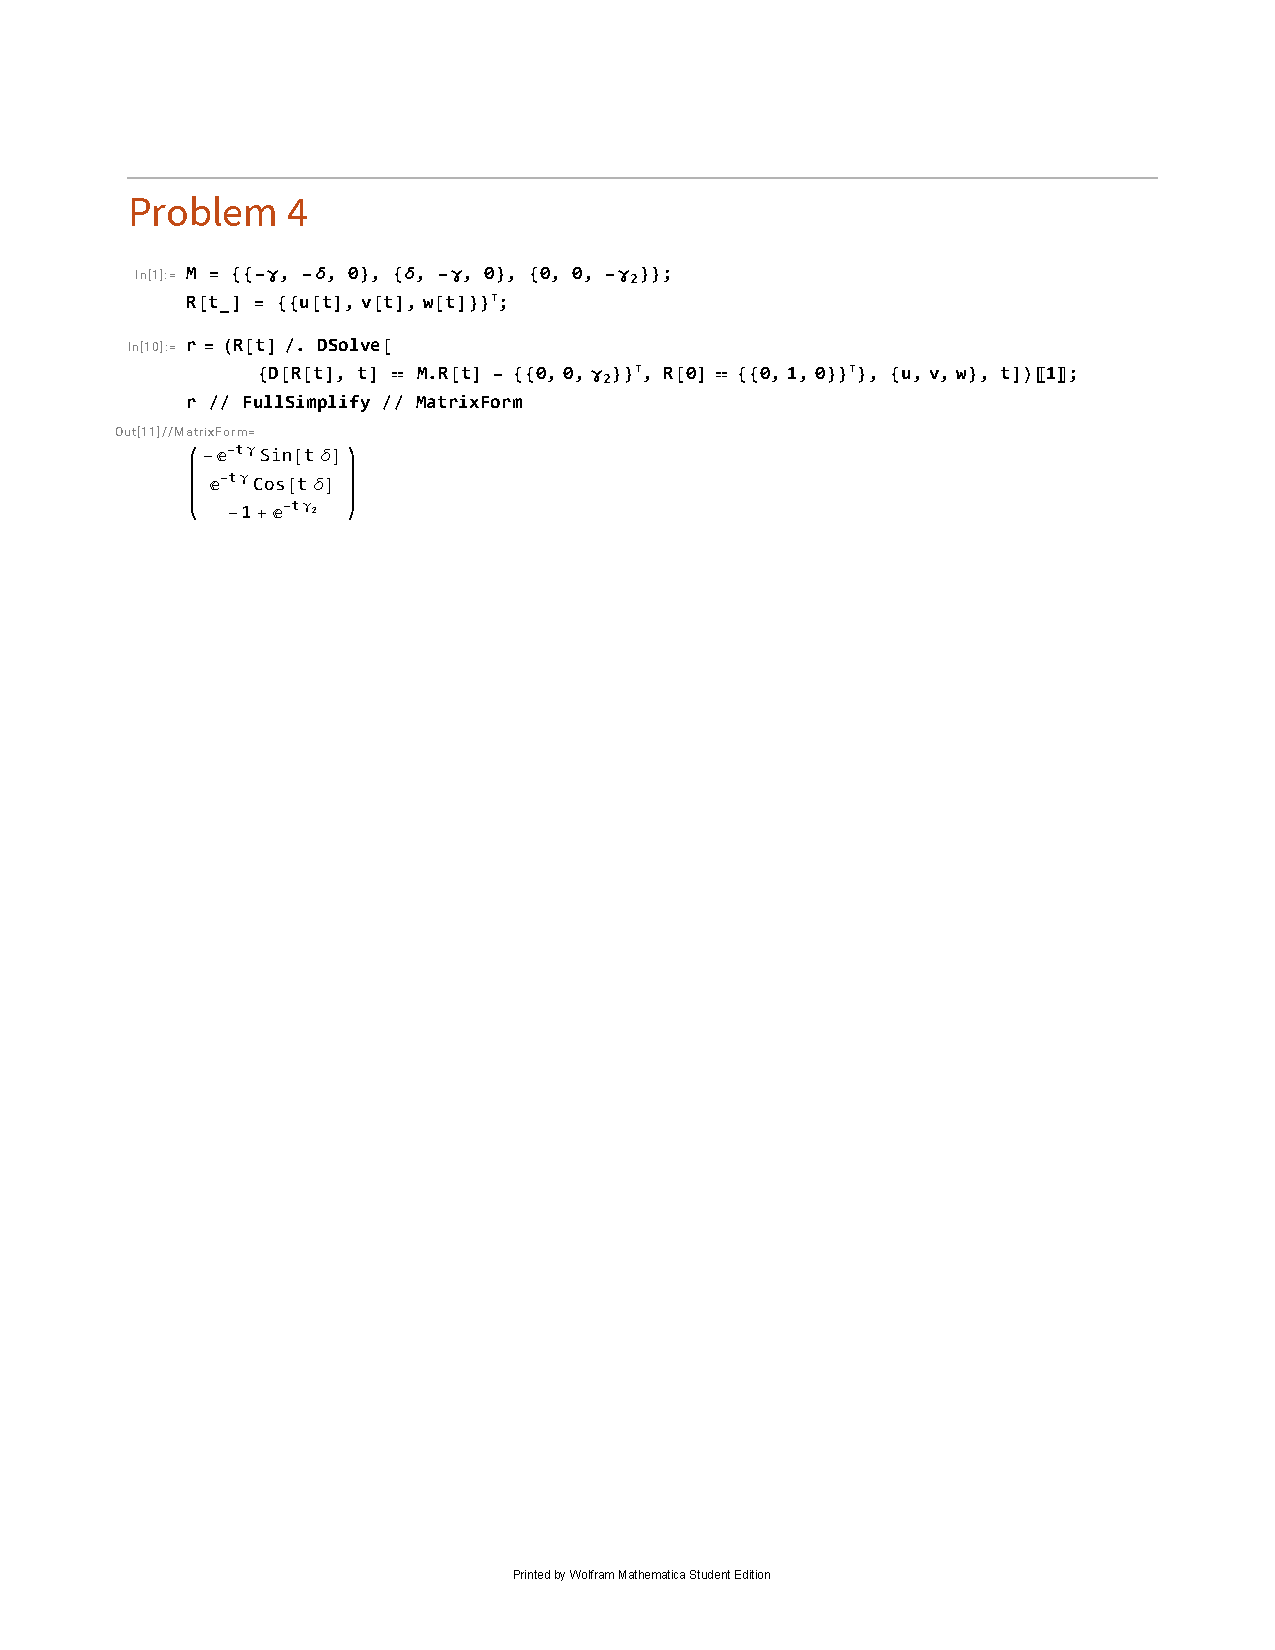
\includepdf[pages=-]{calcs/HW7_mathematica.pdf}
\end{document}